

\documentclass[a4paper,12pt]{report}
\usepackage[utf8]{inputenc}
\usepackage[english]{babel}
\usepackage[T1]{fontenc}
\usepackage{fancyvrb}
\usepackage{url}
\usepackage{alltt}
\usepackage{graphicx}
\usepackage{aeguill}
\usepackage{listings}
\usepackage{verbatim}
\usepackage{a4wide}
\usepackage{indentfirst}
\usepackage{acronym}
\usepackage[hmargin=2cm,vmargin=2cm,bmargin=2cm]{geometry}
\usepackage{color}
\usepackage{float}
\usepackage{tabularx}
\usepackage{multirow}
\usepackage[nottoc,notlof,numbib,notlot]{tocbibind} 
\usepackage{chngcntr}
\usepackage[pdftex]{hyperref}
\usepackage{lastpage}
\usepackage{wrapfig}
\usepackage{bookmark}
\usepackage[table]{xcolor}
\usepackage{color, colortbl}
\usepackage{supertabular}



\counterwithout{figure}{chapter}
\counterwithout{table}{chapter}

% Cabeçalhos e Rodapés
\usepackage{fancyhdr}

\setlength{\headheight}{15pt}



\fancypagestyle{plain}{%
\fancyhead{} % Tirar cabeçalhos de página vazias
\renewcommand{\headrulewidth}{0pt} % e o risco
}

\fancypagestyle{empty}{%
\fancyhead{} % Tirar cabeçalhos de página vazias
\fancyfoot{}
\renewcommand{\headrulewidth}{0pt} % e o risco
\renewcommand{\footrulewidth}{0pt}
}


\usepackage{listings}

\lstset{
  backgroundcolor=\color{white},   	% choose the background color; you must add \usepackage{color} or \usepackage{xcolor}
  belowcaptionskip=\baselineskip,	%
  basicstyle=\small,				% the size of the fonts that are used for the code
  breakatwhitespace=false,         	% sets if automatic breaks should only happen at whitespace
  breaklines=true,                 	% sets automatic line breaking
  captionpos=b,                    	% sets the caption-position to bottom
  commentstyle=\itshape\color{purple!40!black},    	% comment style
  deletekeywords={...},            	% if you want to delete keywords from the given language
  escapeinside={\%*}{*)},          	% if you want to add LaTeX within your code
  extendedchars=true,              	% lets you use non-ASCII characters; for 8-bits encodings only, does not work with UTF-8
  frame=single,                    	% adds a frame around the code
  keywordstyle=\bfseries\color{green!40!black},       	% keyword style		               	% the language of the code
  morekeywords={*,...},            	% if you want to add more keywords to the set
  numbers=none,                    	% where to put the line-numbers; possible values are (none, left, right)
  numbersep=9pt,                   	% how far the line-numbers are from the code
  numberstyle=\tiny\color{mygray}, 	% the style that is used for the line-numbers
  rulecolor=\color{black},         	% if not set, the frame-color may be changed on line-breaks within not-black text (e.g. comments (green here))
  showspaces=false,                	% show spaces everywhere adding particular underscores; it overrides 'showstringspaces'
  showstringspaces=false,          	% underline spaces within strings only
  showtabs=false,                  	% show tabs within strings adding particular underscores
  stepnumber=1,                    	% the step between two line-numbers. If it's 1, each line will be numbered
  stringstyle=\color{orange},     	% string literal style
  tabsize=2		                  	% sets default tabsize to 2 spaces
}
\renewcommand{\lstlistingname}{}


\hypersetup{
   colorlinks,
   citecolor=black,
   filecolor=black,
   linkcolor=black,
   urlcolor=black
}

\title{\begin{center}
\begin{tabular}{c r}
	\large{Universidade do Minho} &\\ 
	\large{Departamento de Informática} &\\
	\large{Mestrado em Engenharia Informática} &\\
	\\
	\large{Metódos Formais em Engenharia de Software} & \\
	\large{Group F} & \\
	\large{Cohesive Project: CSAIL/MIT Proposal} & \\
	\\
	\large{\textbf{ValidAlloy}} &  \\
	\large{\textbf{A tool for validating a git alloy specification using test-case
generation}} & \\
	\\
	 \\
	\end{tabular}
\end{center}}
\author{
\begin{tabular}[t]{c c}
   \multicolumn{2}{c}{Authors:}
	\\
	\\
	 José Pinheiro & Tiago Guimarães \\
	 {\small \texttt{pg23208@di.uminho.pt}}  & {\small \texttt{pg22832@di.uminho.pt}} \\
	\\ 
	\multicolumn{2}{c}{Supervisors:}
	\\
	\\
	Alcino Cunha & Enusuk Kang \\
	 {\small \texttt{alcino@di.uminho.pt}} &{\small \texttt{eskang@csail.mit.edu}} \\
	 \\
	\end{tabular}
}

\begin{document}
%%%
%%% Capa
%%%
\maketitle

%%%
%%% Abstract
%%%

\begin{abstract}
In the world of software, formal models are continually getting more important, but a lot of  software is being built without a formal model to back it up. In this document we will talk about our approach to validate models of existing software, model validation through test case generation, and our tool that implements it. We used git as our case study, mainly because of its popularity and its bad documentation, and worked to get and accurate model of it, and tried to find git bugs while doing it.
\end{abstract}

\tableofcontents
\clearpage

\listoffigures
\clearpage
%%%
%%% Introdução
%%%
\chapter{Introduction}

%
%Introduction
%


\section{Motivation}
\subsection{Git}

 Git\cite{git} is a famous distributed revision control and source code
management system with an emphasis on speed.


One of it's main features is its fast branching and merging. That is because branches in git are very lightweight, a branch in git is only a reference to a single commit.


It has complete history and full revision tracking capabilities;


Its commands are divided into two types:
\begin{itemize}
\item Porcelain commands: The type of commands that the normal user should be using most of the time, very high-level;
\item Plumbling commands: The low-level commands, commonly used for some tweaks.
\end{itemize}

But git is not a perfect world, as we can see by some random internet quotes:

\begin{quote}
``What a pity that it’s so hard to learn, has such an unpleasant command line interface, and treats its users with such utter contempt."
\end{quote}
\begin{flushright}
\textit{\href{http://steveko.wordpress.com/2012/02/24/10-things-i-hate-about-git/}{10 things I hate about Git}}
\end{flushright}

\begin{quote}
``The man pages are one almighty “f*ck you”. They describe the commands from the perspective of a computer scientist, not a user."
\end{quote}
\begin{flushright}
\textit{\href{http://steveko.wordpress.com/2012/02/24/10-things-i-hate-about-git/}{10 things I hate about Git}}

\end{flushright}

\begin{quote}
``(...) there are lots of "cheat sheets" floating around about how to use git tools - I think this is evidence that [...] many
 people have to write "GIT for mortals" pages..."
\end{quote}
\begin{flushright}
\textit{Perl Mailing List}
\end{flushright}


Git is a complex tool, it is not simple to use and its manual is obscure.
Its commands are multi-purpose and sometimes they won't work as you expect them to, or even do something that isn't even mentioned on the manual.


For those reasons, we purpose the creation of a formal git model to alleviate some of these problems.
With an actual git model it would be easier to predict the system behaviour, as well as verify some of the system's properties.
A model would also help with the finding of bugs, because you could say that an operations didn't run as expected by the formal model.
The main problem would be how accurate the model would be. It needs to be validated!


But validating a formal model of an existing system is not a easy task. Deriving the model from the code is a option, just as well as trial and error, our approach is test case generation.

\section{Solution}


Model validation through test case generation is an approach where we use a model to generate test runs with the input of a modelled operation and its expected result, which is then compared with a run of the actual system operation for the same input, if they do not match then the model is not accurate or the system is bugged.

\begin{figure}[H]
\centering
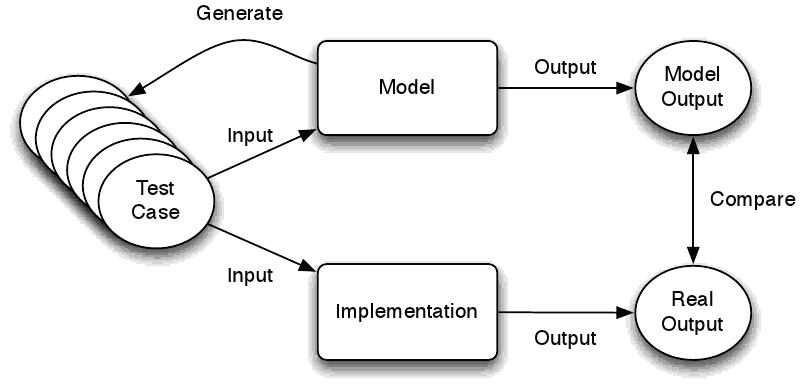
\includegraphics[width=\textwidth]{images/test-case.png}
\caption{Model validation through test case generation}
\end{figure}


We are using a Alloy\cite{alloy} model to represent git, because Alloy provides us the features needed for the use of model validation through test case generation, we can use predicates model the operations and make use of its solving to generate the test cases. It also has a Java API which we used to automate the process.


This approach makes the validation highly automatic, but we must have caution about our pre-conditions strength. Pre-conditions too strong won't fully test the operation and it is hard to recognize when a pre-condition is too strong, so we might miss some bugs.





%%%
%%% Testbench
%%%
\chapter{ValidAlloy}


\documentclass[a4paper,12pt]{report}
\usepackage[utf8]{inputenc}
\usepackage[english]{babel}
\usepackage[T1]{fontenc}
\usepackage{fancyvrb}
\usepackage{url}
\usepackage{alltt}
\usepackage{graphicx}
\usepackage{aeguill}
\usepackage{listings}
\usepackage{verbatim}
\usepackage{a4wide}
\usepackage{indentfirst}
\usepackage{acronym}
\usepackage[hmargin=2cm,vmargin=2cm,bmargin=2cm]{geometry}
\usepackage{color}
\usepackage{float}
\usepackage{tabularx}
\usepackage{multirow}
\usepackage[nottoc,notlof,numbib,notlot]{tocbibind} 
\usepackage{chngcntr}
\usepackage[pdftex]{hyperref}
\usepackage{lastpage}
\usepackage{wrapfig}
\usepackage{bookmark}
\usepackage[table]{xcolor}
\usepackage{color, colortbl}
\usepackage{supertabular}



\counterwithout{figure}{chapter}
\counterwithout{table}{chapter}

% Cabeçalhos e Rodapés
\usepackage{fancyhdr}

\setlength{\headheight}{15pt}



\fancypagestyle{plain}{%
\fancyhead{} % Tirar cabeçalhos de página vazias
\renewcommand{\headrulewidth}{0pt} % e o risco
}

\fancypagestyle{empty}{%
\fancyhead{} % Tirar cabeçalhos de página vazias
\fancyfoot{}
\renewcommand{\headrulewidth}{0pt} % e o risco
\renewcommand{\footrulewidth}{0pt}
}


\usepackage{listings}

\lstset{
  backgroundcolor=\color{white},   	% choose the background color; you must add \usepackage{color} or \usepackage{xcolor}
  belowcaptionskip=\baselineskip,	%
  basicstyle=\small,				% the size of the fonts that are used for the code
  breakatwhitespace=false,         	% sets if automatic breaks should only happen at whitespace
  breaklines=true,                 	% sets automatic line breaking
  captionpos=b,                    	% sets the caption-position to bottom
  commentstyle=\itshape\color{purple!40!black},    	% comment style
  deletekeywords={...},            	% if you want to delete keywords from the given language
  escapeinside={\%*}{*)},          	% if you want to add LaTeX within your code
  extendedchars=true,              	% lets you use non-ASCII characters; for 8-bits encodings only, does not work with UTF-8
  frame=single,                    	% adds a frame around the code
  keywordstyle=\bfseries\color{green!40!black},       	% keyword style		               	% the language of the code
  morekeywords={*,...},            	% if you want to add more keywords to the set
  numbers=none,                    	% where to put the line-numbers; possible values are (none, left, right)
  numbersep=9pt,                   	% how far the line-numbers are from the code
  numberstyle=\tiny\color{mygray}, 	% the style that is used for the line-numbers
  rulecolor=\color{black},         	% if not set, the frame-color may be changed on line-breaks within not-black text (e.g. comments (green here))
  showspaces=false,                	% show spaces everywhere adding particular underscores; it overrides 'showstringspaces'
  showstringspaces=false,          	% underline spaces within strings only
  showtabs=false,                  	% show tabs within strings adding particular underscores
  stepnumber=1,                    	% the step between two line-numbers. If it's 1, each line will be numbered
  stringstyle=\color{orange},     	% string literal style
  tabsize=2		                  	% sets default tabsize to 2 spaces
}
\renewcommand{\lstlistingname}{}


\hypersetup{
   colorlinks,
   citecolor=black,
   filecolor=black,
   linkcolor=black,
   urlcolor=black
}

\title{\begin{center}
\begin{tabular}{c r}
	\large{Universidade do Minho} &\\ 
	\large{Departamento de Informática} &\\
	\large{Mestrado em Engenharia Informática} &\\
	\\
	\large{Metódos Formais em Engenharia de Software} & \\
	\large{Group F} & \\
	\large{Cohesive Project: CSAIL/MIT Proposal} & \\
	\\
	\large{\textbf{ValidAlloy}} &  \\
	\large{\textbf{A tool for validating a git alloy specification using test-case
generation}} & \\
	\\
	 \\
	\end{tabular}
\end{center}}
\author{
\begin{tabular}[t]{c c}
   \multicolumn{2}{c}{Authors:}
	\\
	\\
	 José Pinheiro & Tiago Guimarães \\
	 {\small \texttt{pg23208@di.uminho.pt}}  & {\small \texttt{pg22832@di.uminho.pt}} \\
	\\ 
	\multicolumn{2}{c}{Supervisors:}
	\\
	\\
	Alcino Cunha & Enusuk Kang \\
	 {\small \texttt{alcino@di.uminho.pt}} &{\small \texttt{eskang@csail.mit.edu}} \\
	 \\
	\end{tabular}
}

\begin{document}
%%%
%%% Capa
%%%
\maketitle

%%%
%%% Abstract
%%%

\begin{abstract}
In the world of software, formal models are continually getting more important, but a lot of  software is being built without a formal model to back it up. In this document we will talk about our approach to validate models of existing software, model validation through test case generation, and our tool that implements it. We used git as our case study, mainly because of its popularity and its bad documentation, and worked to get and accurate model of it, and tried to find git bugs while doing it.
\end{abstract}

\tableofcontents
\clearpage

\listoffigures
\clearpage
%%%
%%% Introdução
%%%
\chapter{Introduction}

%
%Introduction
%


\section{Motivation}
\subsection{Git}

 Git\cite{git} is a famous distributed revision control and source code
management system with an emphasis on speed.


One of it's main features is its fast branching and merging. That is because branches in git are very lightweight, a branch in git is only a reference to a single commit.


It has complete history and full revision tracking capabilities;


Its commands are divided into two types:
\begin{itemize}
\item Porcelain commands: The type of commands that the normal user should be using most of the time, very high-level;
\item Plumbling commands: The low-level commands, commonly used for some tweaks.
\end{itemize}

But git is not a perfect world, as we can see by some random internet quotes:

\begin{quote}
``What a pity that it’s so hard to learn, has such an unpleasant command line interface, and treats its users with such utter contempt."
\end{quote}
\begin{flushright}
\textit{\href{http://steveko.wordpress.com/2012/02/24/10-things-i-hate-about-git/}{10 things I hate about Git}}
\end{flushright}

\begin{quote}
``The man pages are one almighty “f*ck you”. They describe the commands from the perspective of a computer scientist, not a user."
\end{quote}
\begin{flushright}
\textit{\href{http://steveko.wordpress.com/2012/02/24/10-things-i-hate-about-git/}{10 things I hate about Git}}

\end{flushright}

\begin{quote}
``(...) there are lots of "cheat sheets" floating around about how to use git tools - I think this is evidence that [...] many
 people have to write "GIT for mortals" pages..."
\end{quote}
\begin{flushright}
\textit{Perl Mailing List}
\end{flushright}


Git is a complex tool, it is not simple to use and its manual is obscure.
Its commands are multi-purpose and sometimes they won't work as you expect them to, or even do something that isn't even mentioned on the manual.


For those reasons, we purpose the creation of a formal git model to alleviate some of these problems.
With an actual git model it would be easier to predict the system behaviour, as well as verify some of the system's properties.
A model would also help with the finding of bugs, because you could say that an operations didn't run as expected by the formal model.
The main problem would be how accurate the model would be. It needs to be validated!


But validating a formal model of an existing system is not a easy task. Deriving the model from the code is a option, just as well as trial and error, our approach is test case generation.

\section{Solution}


Model validation through test case generation is an approach where we use a model to generate test runs with the input of a modelled operation and its expected result, which is then compared with a run of the actual system operation for the same input, if they do not match then the model is not accurate or the system is bugged.

\begin{figure}[H]
\centering
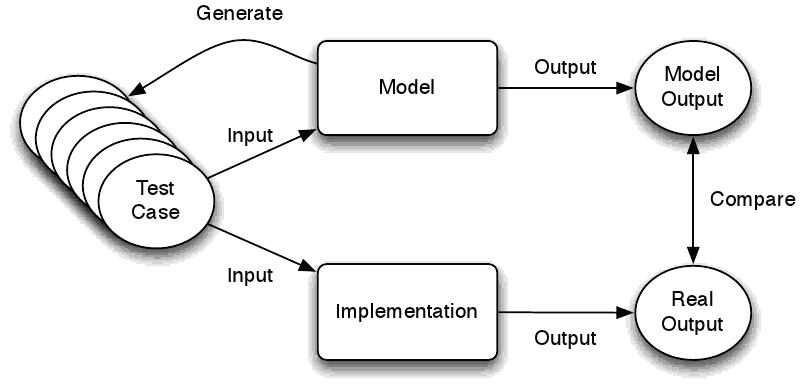
\includegraphics[width=\textwidth]{images/test-case.png}
\caption{Model validation through test case generation}
\end{figure}


We are using a Alloy\cite{alloy} model to represent git, because Alloy provides us the features needed for the use of model validation through test case generation, we can use predicates model the operations and make use of its solving to generate the test cases. It also has a Java API which we used to automate the process.


This approach makes the validation highly automatic, but we must have caution about our pre-conditions strength. Pre-conditions too strong won't fully test the operation and it is hard to recognize when a pre-condition is too strong, so we might miss some bugs.





%%%
%%% Testbench
%%%
\chapter{ValidAlloy}


\documentclass[a4paper,12pt]{report}
\usepackage[utf8]{inputenc}
\usepackage[english]{babel}
\usepackage[T1]{fontenc}
\usepackage{fancyvrb}
\usepackage{url}
\usepackage{alltt}
\usepackage{graphicx}
\usepackage{aeguill}
\usepackage{listings}
\usepackage{verbatim}
\usepackage{a4wide}
\usepackage{indentfirst}
\usepackage{acronym}
\usepackage[hmargin=2cm,vmargin=2cm,bmargin=2cm]{geometry}
\usepackage{color}
\usepackage{float}
\usepackage{tabularx}
\usepackage{multirow}
\usepackage[nottoc,notlof,numbib,notlot]{tocbibind} 
\usepackage{chngcntr}
\usepackage[pdftex]{hyperref}
\usepackage{lastpage}
\usepackage{wrapfig}
\usepackage{bookmark}
\usepackage[table]{xcolor}
\usepackage{color, colortbl}
\usepackage{supertabular}



\counterwithout{figure}{chapter}
\counterwithout{table}{chapter}

% Cabeçalhos e Rodapés
\usepackage{fancyhdr}

\setlength{\headheight}{15pt}



\fancypagestyle{plain}{%
\fancyhead{} % Tirar cabeçalhos de página vazias
\renewcommand{\headrulewidth}{0pt} % e o risco
}

\fancypagestyle{empty}{%
\fancyhead{} % Tirar cabeçalhos de página vazias
\fancyfoot{}
\renewcommand{\headrulewidth}{0pt} % e o risco
\renewcommand{\footrulewidth}{0pt}
}


\usepackage{listings}

\lstset{
  backgroundcolor=\color{white},   	% choose the background color; you must add \usepackage{color} or \usepackage{xcolor}
  belowcaptionskip=\baselineskip,	%
  basicstyle=\small,				% the size of the fonts that are used for the code
  breakatwhitespace=false,         	% sets if automatic breaks should only happen at whitespace
  breaklines=true,                 	% sets automatic line breaking
  captionpos=b,                    	% sets the caption-position to bottom
  commentstyle=\itshape\color{purple!40!black},    	% comment style
  deletekeywords={...},            	% if you want to delete keywords from the given language
  escapeinside={\%*}{*)},          	% if you want to add LaTeX within your code
  extendedchars=true,              	% lets you use non-ASCII characters; for 8-bits encodings only, does not work with UTF-8
  frame=single,                    	% adds a frame around the code
  keywordstyle=\bfseries\color{green!40!black},       	% keyword style		               	% the language of the code
  morekeywords={*,...},            	% if you want to add more keywords to the set
  numbers=none,                    	% where to put the line-numbers; possible values are (none, left, right)
  numbersep=9pt,                   	% how far the line-numbers are from the code
  numberstyle=\tiny\color{mygray}, 	% the style that is used for the line-numbers
  rulecolor=\color{black},         	% if not set, the frame-color may be changed on line-breaks within not-black text (e.g. comments (green here))
  showspaces=false,                	% show spaces everywhere adding particular underscores; it overrides 'showstringspaces'
  showstringspaces=false,          	% underline spaces within strings only
  showtabs=false,                  	% show tabs within strings adding particular underscores
  stepnumber=1,                    	% the step between two line-numbers. If it's 1, each line will be numbered
  stringstyle=\color{orange},     	% string literal style
  tabsize=2		                  	% sets default tabsize to 2 spaces
}
\renewcommand{\lstlistingname}{}


\hypersetup{
   colorlinks,
   citecolor=black,
   filecolor=black,
   linkcolor=black,
   urlcolor=black
}

\title{\begin{center}
\begin{tabular}{c r}
	\large{Universidade do Minho} &\\ 
	\large{Departamento de Informática} &\\
	\large{Mestrado em Engenharia Informática} &\\
	\\
	\large{Metódos Formais em Engenharia de Software} & \\
	\large{Group F} & \\
	\large{Cohesive Project: CSAIL/MIT Proposal} & \\
	\\
	\large{\textbf{ValidAlloy}} &  \\
	\large{\textbf{A tool for validating a git alloy specification using test-case
generation}} & \\
	\\
	 \\
	\end{tabular}
\end{center}}
\author{
\begin{tabular}[t]{c c}
   \multicolumn{2}{c}{Authors:}
	\\
	\\
	 José Pinheiro & Tiago Guimarães \\
	 {\small \texttt{pg23208@di.uminho.pt}}  & {\small \texttt{pg22832@di.uminho.pt}} \\
	\\ 
	\multicolumn{2}{c}{Supervisors:}
	\\
	\\
	Alcino Cunha & Enusuk Kang \\
	 {\small \texttt{alcino@di.uminho.pt}} &{\small \texttt{eskang@csail.mit.edu}} \\
	 \\
	\end{tabular}
}

\begin{document}
%%%
%%% Capa
%%%
\maketitle

%%%
%%% Abstract
%%%

\begin{abstract}
In the world of software, formal models are continually getting more important, but a lot of  software is being built without a formal model to back it up. In this document we will talk about our approach to validate models of existing software, model validation through test case generation, and our tool that implements it. We used git as our case study, mainly because of its popularity and its bad documentation, and worked to get and accurate model of it, and tried to find git bugs while doing it.
\end{abstract}

\tableofcontents
\clearpage

\listoffigures
\clearpage
%%%
%%% Introdução
%%%
\chapter{Introduction}

%
%Introduction
%


\section{Motivation}
\subsection{Git}

 Git\cite{git} is a famous distributed revision control and source code
management system with an emphasis on speed.


One of it's main features is its fast branching and merging. That is because branches in git are very lightweight, a branch in git is only a reference to a single commit.


It has complete history and full revision tracking capabilities;


Its commands are divided into two types:
\begin{itemize}
\item Porcelain commands: The type of commands that the normal user should be using most of the time, very high-level;
\item Plumbling commands: The low-level commands, commonly used for some tweaks.
\end{itemize}

But git is not a perfect world, as we can see by some random internet quotes:

\begin{quote}
``What a pity that it’s so hard to learn, has such an unpleasant command line interface, and treats its users with such utter contempt."
\end{quote}
\begin{flushright}
\textit{\href{http://steveko.wordpress.com/2012/02/24/10-things-i-hate-about-git/}{10 things I hate about Git}}
\end{flushright}

\begin{quote}
``The man pages are one almighty “f*ck you”. They describe the commands from the perspective of a computer scientist, not a user."
\end{quote}
\begin{flushright}
\textit{\href{http://steveko.wordpress.com/2012/02/24/10-things-i-hate-about-git/}{10 things I hate about Git}}

\end{flushright}

\begin{quote}
``(...) there are lots of "cheat sheets" floating around about how to use git tools - I think this is evidence that [...] many
 people have to write "GIT for mortals" pages..."
\end{quote}
\begin{flushright}
\textit{Perl Mailing List}
\end{flushright}


Git is a complex tool, it is not simple to use and its manual is obscure.
Its commands are multi-purpose and sometimes they won't work as you expect them to, or even do something that isn't even mentioned on the manual.


For those reasons, we purpose the creation of a formal git model to alleviate some of these problems.
With an actual git model it would be easier to predict the system behaviour, as well as verify some of the system's properties.
A model would also help with the finding of bugs, because you could say that an operations didn't run as expected by the formal model.
The main problem would be how accurate the model would be. It needs to be validated!


But validating a formal model of an existing system is not a easy task. Deriving the model from the code is a option, just as well as trial and error, our approach is test case generation.

\section{Solution}


Model validation through test case generation is an approach where we use a model to generate test runs with the input of a modelled operation and its expected result, which is then compared with a run of the actual system operation for the same input, if they do not match then the model is not accurate or the system is bugged.

\begin{figure}[H]
\centering
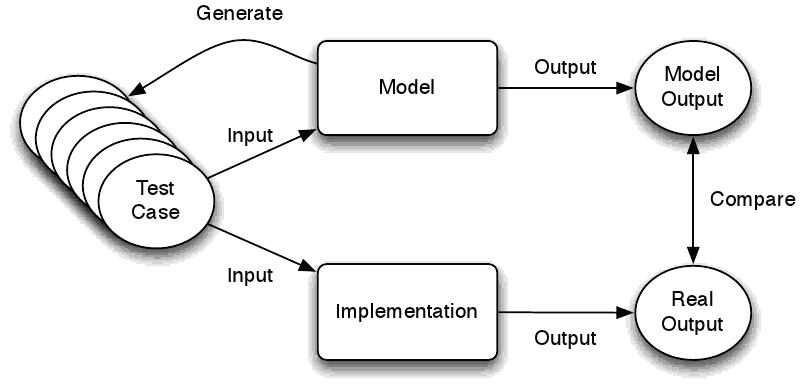
\includegraphics[width=\textwidth]{images/test-case.png}
\caption{Model validation through test case generation}
\end{figure}


We are using a Alloy\cite{alloy} model to represent git, because Alloy provides us the features needed for the use of model validation through test case generation, we can use predicates model the operations and make use of its solving to generate the test cases. It also has a Java API which we used to automate the process.


This approach makes the validation highly automatic, but we must have caution about our pre-conditions strength. Pre-conditions too strong won't fully test the operation and it is hard to recognize when a pre-condition is too strong, so we might miss some bugs.





%%%
%%% Testbench
%%%
\chapter{ValidAlloy}


\input{sections/Setup.tex}
\begin{document}
%%%
%%% Capa
%%%
\maketitle

%%%
%%% Abstract
%%%

\begin{abstract}
In the world of software, formal models are continually getting more important, but a lot of  software is being built without a formal model to back it up. In this document we will talk about our approach to validate models of existing software, model validation through test case generation, and our tool that implements it. We used git as our case study, mainly because of its popularity and its bad documentation, and worked to get and accurate model of it, and tried to find git bugs while doing it.
\end{abstract}

\tableofcontents
\clearpage

\listoffigures
\clearpage
%%%
%%% Introdução
%%%
\chapter{Introduction}

\input{sections/introduction.tex}

%%%
%%% Testbench
%%%
\chapter{ValidAlloy}
\input{sections/validAlloy.tex}

%%%
%%% Implementação
%%%

\chapter{Results}
\input{sections/results.tex}
%%%
%%% Últimas observações gerais (?)
%%%

\chapter{Conclusions}
Git is not nearly perfect, its documentation is incomplete, and the functionality of some operations makes it hard to understand what they actually do. 
We are satisfied with model validation through test case generation, on the simpler commands it showed not apparent errors, and on the complex one it provided us some really weird behaviour, as it should be expected. 
We believed that we used this well to validate our model, and to create and run all those tests, and we found an actual bug in git. But there are still some problems: model depth limits how accurate the tests are. And of course, you must be good with modelling to use it well.
You can check out our work at \href{https://github.com/eskang/validAlloy}{https://github.com/eskang/validAlloy}.

\chapter{Possible future work}

After this, we believe that there is some work can still to be done. The model needs to be refined, and there are some operations that are yet to be done( merge and commit for example). The testbench needs an update on the documentation(we are working on it).
We also believe that it should be possible to create a framework to make testbenches, like this one that use alloy and the test case generation approach. We believe to a big part of the work could be saved.

\begin{thebibliography}{9}

\bibitem{alloy}
  Official alloy website, \href{http://alloy.mit.edu/}{http://alloy.mit.edu/}.

\bibitem{git}
	Official git website, \href{http://git-scm.com/}{http://git-scm.com/}.


\bibitem{gitpro}
  Scott Chacon,
  \emph{Pro Git}.
  Apress, Berkely, CA, USA
  2009.
  
\bibitem{git_man}
	Git man pages, \href{https://www.kernel.org/pub/software/scm/git/docs/}{https://www.kernel.org/pub/software/scm/git/docs/}.


\bibitem{git_mail}
Discussion of the git rm bug, \href{http://git.661346.n2.nabble.com/Behavior-of-git-rm-td7581485.html}{http://git.661346.n2.nabble.com/Behavior-of-git-rm-td7581485.html}.

\bibitem{antlr}
Official antlr website, \href{www.antlr.org}{www.antlr.org}.

\end{thebibliography}

\appendix
\cleardoublepage
\phantomsection
\addcontentsline{toc}{chapter}{\appendixname}

\chapter{Config File Grammar}
\input{sections/appendix/grammar.tex}

\end{document}

%%%
%%% Implementação
%%%

\chapter{Results}

The model we used is a legacy one, and it describes the file system and the git objects(blob, tree, commit, tag), index and heads(including the HEAD).
We modelled the git add,branch and remove operations and tested them with our testbench, the results follows.

\section{Git add}

Git add is used to track files and fix merge conflicts. Or Alloy model is too abstract, we don't have on our modelled index, the information need for merge and its conflicts, so we are only testing the tracking part of git add. With this in mind, git add becomes a rather simple operation that just puts the files on the index if they are not already there. With our current Testbench we couldn't find any difference.

\begin{lstlisting}[caption=Predicate add]
pred add [s,s' : State,p : Path] {
	s != s'
	p in (node.s).path
	path.p in File
	object.s' = object.s + (path.p).blob
	index.s' = index.s ++ p->(path.p).blob
 	ref.s' = ref.s
	head.s' = head.s
	HEAD.s' = HEAD.s
	node.s' = node.s
}
\end{lstlisting}
\newpage
\section{Git branch}
Git branch's speed is one of git's selling points. Its speed comes from is simplicity, branching in git is just creating another pointer to the actual commit. So its post-conditions are not that complicated, and its pre-conditions are also simple: you cannot branch before your first commit, and you can't give the new branch the same name as an existing one.


Our approach could not find any problems with git branch. And we also believe that git branch is fine, specially because of its simplicity.


\begin{lstlisting}[caption=Predicate branch]
pred branchPC[s:State, b:Ref]
{
	some (HEAD.s).head.s
	b not in (head.s).univ
}



pred gitBranch[s,s': State , n:Ref ]{

	branchPC[s,n]

	head.s' = head.s +  (n->((HEAD.s).head.s))
	
	HEAD.s' = HEAD.s	
	object.s' = object.s
	node.s' = node.s
	index.s' = index.s
}

\end{lstlisting}

\section{Git rm}

Git remote, according to the man pages, should remove the entry of a file from the index and, if it exists on the file system, deletes it. But with our testbench we fond out that if a file is the last one in a directory,when you remove it with git remove, it will also delete the containing directory and every other ancestor directory that also becomes empty, this is unmentioned on the man pages and on the Git Pro Manual.


Git manual states that the files being removed have to be identical to the tip of the branch and no updates to their contents can be staged in the index. But we noted that sometimes git remove would run even if one of this conditions didn't hold, so we decided to test when some of the pre-condition don't hold as well.This was the motivation to the error expecting part of the testbench, so that we wouldn't get our results spammed with the expected result of a negated pre-condtion.


With this our approach to this operation became:
\begin{itemize}
\item Run git rm with both pre-conditions holding true;
\item Negate one pre-condition alternatively and test, while the other held true;
\item Test with both pre-conditions being false.
\end{itemize}

\begin{lstlisting}[caption=Predicate rm]
pred rmConditionA[s:State,p:Path]{
		(((HEAD.s).head.s).path.s).p & Blob = (path.p & node.s).blob
}

pred rmConditionB[s:State,p:Path]{
	  p.index.s in (((HEAD.s).head.s).path.s).p 
}
pred rmAB[s,s':State,p:Path]{
	rmConditionA[s,p]
	rmConditionB[s,p]
	rmBehaviour[s,s',p]
}

pred rmA[s,s':State,p:Path]{
	rmConditionA[s,p]
	not rmConditionB[s,p]
	rmBehaviour[s,s',p]
}

pred rmB[s,s':State,p:Path]{
	not rmConditionA[s,p]
	rmConditionB[s,p]
	rmBehaviour[s,s',p]
}

pred rmNOP[s,s':State,p:Path]{
	not rmConditionA[s,p]
	not rmConditionB[s,p]
	rmBehaviour[s,s',p]
}

pred rmBehaviour[s,s':State,p:Path]{
	p in (index.s).univ
	some path.p & node.s => some path.(p.siblings) & node.s 
	path.p in File & node.s 
	index.s' = index.s - p->Blob
	node.s' = node.s - path.p
	object.s' = object.s
	head.s' = head.s
	HEAD.s' = HEAD.s
}
\end{lstlisting}

With this approach we where able to identify a weird error that could be replicated with this trace:
\begin{verbatim}
$ git init
$ mkdir D
$ echo "Hi" > D/F
$ git add D/F
$ rm -r D
$ echo "Hey" > D
$ git rm D/F
warning : ’D/F’: Not a directory
rm ’D/F’
fatal: git rm: ’D/F’: Not a directory
\end{verbatim}



If we instead did:

\begin{verbatim}
$ git init
$ mkdir D
$ echo "Hi" > D/F
$ git add D/F
$ rm -r D
$ echo "Hey" > F
$ git rm D/F
\end{verbatim}
This works as expected.


We asked at git@vger.kernel.org\cite{git_mail}, if this was the correct behaviour from git rm, in the first reply, they suggested a patch for it. It should also be noted that because of our post they also identified a similar problem but with symbolic links instead of files, that could cause some trouble.

%%%
%%% Últimas observações gerais (?)
%%%

\chapter{Conclusions}
Git is not nearly perfect, its documentation is incomplete, and the functionality of some operations makes it hard to understand what they actually do. 
We are satisfied with model validation through test case generation, on the simpler commands it showed not apparent errors, and on the complex one it provided us some really weird behaviour, as it should be expected. 
We believed that we used this well to validate our model, and to create and run all those tests, and we found an actual bug in git. But there are still some problems: model depth limits how accurate the tests are. And of course, you must be good with modelling to use it well.
You can check out our work at \href{https://github.com/eskang/validAlloy}{https://github.com/eskang/validAlloy}.

\chapter{Possible future work}

After this, we believe that there is some work can still to be done. The model needs to be refined, and there are some operations that are yet to be done( merge and commit for example). The testbench needs an update on the documentation(we are working on it).
We also believe that it should be possible to create a framework to make testbenches, like this one that use alloy and the test case generation approach. We believe to a big part of the work could be saved.

\begin{thebibliography}{9}

\bibitem{alloy}
  Official alloy website, \href{http://alloy.mit.edu/}{http://alloy.mit.edu/}.

\bibitem{git}
	Official git website, \href{http://git-scm.com/}{http://git-scm.com/}.


\bibitem{gitpro}
  Scott Chacon,
  \emph{Pro Git}.
  Apress, Berkely, CA, USA
  2009.
  
\bibitem{git_man}
	Git man pages, \href{https://www.kernel.org/pub/software/scm/git/docs/}{https://www.kernel.org/pub/software/scm/git/docs/}.


\bibitem{git_mail}
Discussion of the git rm bug, \href{http://git.661346.n2.nabble.com/Behavior-of-git-rm-td7581485.html}{http://git.661346.n2.nabble.com/Behavior-of-git-rm-td7581485.html}.

\bibitem{antlr}
Official antlr website, \href{www.antlr.org}{www.antlr.org}.

\end{thebibliography}

\appendix
\cleardoublepage
\phantomsection
\addcontentsline{toc}{chapter}{\appendixname}

\chapter{Config File Grammar}

Here follows a formal description of the grammar that recognizes the config file language. It is in extendBNF notion.

\begin{verbatim}

cfg 
    : command ( ';' b=command)* runs
    ;	


command   
    : vars? 'pred' pred  'scope'  sp 'cmd'  cmdgit   errors?
    ; 

errors
    :'errors' '(' list_errors ')'
    ;	

list_errors
    :error (','error)*
    ;

error
    :STRING
    ;

runs  
    : 'runs' INT
    ;
	
vars
    : var  (var )*
    ;
	
pred 
    : name arguments
    ;
	

arguments
    :'[' args? ']'
    ;

args 
    :arg (',' arg)*
    ;


sp  
    : 'for'  INT  sigs
    | 'for' INT  'but exactly' sigs
    ;
	
sigs  
    : sig (',' sig )*
    ;
	
sig
    :INT  ID
    ;

var
    :arg ':' type
    ;
	
type 
    :ID
    ;
	
cmdgit
    :'git' name opts
    ;

opts 
    :opt  (opt )*	
    ;
	
opt 
    : ID 
    |arg
    |STRING
    ;
	
	
name 
    : ID
    ;
	
arg
    :'#'ID
    ;
	
ID  :	('a'..'z'|'A'..'Z'|'_'|'-') ('a'..'z'|'A'..'Z'|'0'..'9'|'_'|'-')*
    ;

INT :	'0'..'9'+
    ;

WS  :   ( ' '
        | '\t'
        | '\r'
        | '\n'
        ) {$channel=HIDDEN;}
    ;

STRING
    :  '"' ( ESC_SEQ | ~('\\'|'"') )* '"'
    ;

CHAR:  '\'' ( ESC_SEQ | ~('\''|'\\') ) '\''
    ;

fragment
HEX_DIGIT : ('0'..'9'|'a'..'f'|'A'..'F') ;

fragment
ESC_SEQ
    :   '\\' ('b'|'t'|'n'|'f'|'r'|'\"'|'\''|'\\')
    |   UNICODE_ESC
    |   OCTAL_ESC
    ;

fragment
OCTAL_ESC
    :   '\\' ('0'..'3') ('0'..'7') ('0'..'7')
    |   '\\' ('0'..'7') ('0'..'7')
    |   '\\' ('0'..'7')
    ;

fragment
UNICODE_ESC
    :   '\\' 'u' HEX_DIGIT HEX_DIGIT HEX_DIGIT HEX_DIGIT
    ;
\end{verbatim}

\end{document}

%%%
%%% Implementação
%%%

\chapter{Results}

The model we used is a legacy one, and it describes the file system and the git objects(blob, tree, commit, tag), index and heads(including the HEAD).
We modelled the git add,branch and remove operations and tested them with our testbench, the results follows.

\section{Git add}

Git add is used to track files and fix merge conflicts. Or Alloy model is too abstract, we don't have on our modelled index, the information need for merge and its conflicts, so we are only testing the tracking part of git add. With this in mind, git add becomes a rather simple operation that just puts the files on the index if they are not already there. With our current Testbench we couldn't find any difference.

\begin{lstlisting}[caption=Predicate add]
pred add [s,s' : State,p : Path] {
	s != s'
	p in (node.s).path
	path.p in File
	object.s' = object.s + (path.p).blob
	index.s' = index.s ++ p->(path.p).blob
 	ref.s' = ref.s
	head.s' = head.s
	HEAD.s' = HEAD.s
	node.s' = node.s
}
\end{lstlisting}
\newpage
\section{Git branch}
Git branch's speed is one of git's selling points. Its speed comes from is simplicity, branching in git is just creating another pointer to the actual commit. So its post-conditions are not that complicated, and its pre-conditions are also simple: you cannot branch before your first commit, and you can't give the new branch the same name as an existing one.


Our approach could not find any problems with git branch. And we also believe that git branch is fine, specially because of its simplicity.


\begin{lstlisting}[caption=Predicate branch]
pred branchPC[s:State, b:Ref]
{
	some (HEAD.s).head.s
	b not in (head.s).univ
}



pred gitBranch[s,s': State , n:Ref ]{

	branchPC[s,n]

	head.s' = head.s +  (n->((HEAD.s).head.s))
	
	HEAD.s' = HEAD.s	
	object.s' = object.s
	node.s' = node.s
	index.s' = index.s
}

\end{lstlisting}

\section{Git rm}

Git remote, according to the man pages, should remove the entry of a file from the index and, if it exists on the file system, deletes it. But with our testbench we fond out that if a file is the last one in a directory,when you remove it with git remove, it will also delete the containing directory and every other ancestor directory that also becomes empty, this is unmentioned on the man pages and on the Git Pro Manual.


Git manual states that the files being removed have to be identical to the tip of the branch and no updates to their contents can be staged in the index. But we noted that sometimes git remove would run even if one of this conditions didn't hold, so we decided to test when some of the pre-condition don't hold as well.This was the motivation to the error expecting part of the testbench, so that we wouldn't get our results spammed with the expected result of a negated pre-condtion.


With this our approach to this operation became:
\begin{itemize}
\item Run git rm with both pre-conditions holding true;
\item Negate one pre-condition alternatively and test, while the other held true;
\item Test with both pre-conditions being false.
\end{itemize}

\begin{lstlisting}[caption=Predicate rm]
pred rmConditionA[s:State,p:Path]{
		(((HEAD.s).head.s).path.s).p & Blob = (path.p & node.s).blob
}

pred rmConditionB[s:State,p:Path]{
	  p.index.s in (((HEAD.s).head.s).path.s).p 
}
pred rmAB[s,s':State,p:Path]{
	rmConditionA[s,p]
	rmConditionB[s,p]
	rmBehaviour[s,s',p]
}

pred rmA[s,s':State,p:Path]{
	rmConditionA[s,p]
	not rmConditionB[s,p]
	rmBehaviour[s,s',p]
}

pred rmB[s,s':State,p:Path]{
	not rmConditionA[s,p]
	rmConditionB[s,p]
	rmBehaviour[s,s',p]
}

pred rmNOP[s,s':State,p:Path]{
	not rmConditionA[s,p]
	not rmConditionB[s,p]
	rmBehaviour[s,s',p]
}

pred rmBehaviour[s,s':State,p:Path]{
	p in (index.s).univ
	some path.p & node.s => some path.(p.siblings) & node.s 
	path.p in File & node.s 
	index.s' = index.s - p->Blob
	node.s' = node.s - path.p
	object.s' = object.s
	head.s' = head.s
	HEAD.s' = HEAD.s
}
\end{lstlisting}

With this approach we where able to identify a weird error that could be replicated with this trace:
\begin{verbatim}
$ git init
$ mkdir D
$ echo "Hi" > D/F
$ git add D/F
$ rm -r D
$ echo "Hey" > D
$ git rm D/F
warning : ’D/F’: Not a directory
rm ’D/F’
fatal: git rm: ’D/F’: Not a directory
\end{verbatim}



If we instead did:

\begin{verbatim}
$ git init
$ mkdir D
$ echo "Hi" > D/F
$ git add D/F
$ rm -r D
$ echo "Hey" > F
$ git rm D/F
\end{verbatim}
This works as expected.


We asked at git@vger.kernel.org\cite{git_mail}, if this was the correct behaviour from git rm, in the first reply, they suggested a patch for it. It should also be noted that because of our post they also identified a similar problem but with symbolic links instead of files, that could cause some trouble.

%%%
%%% Últimas observações gerais (?)
%%%

\chapter{Conclusions}
Git is not nearly perfect, its documentation is incomplete, and the functionality of some operations makes it hard to understand what they actually do. 
We are satisfied with model validation through test case generation, on the simpler commands it showed not apparent errors, and on the complex one it provided us some really weird behaviour, as it should be expected. 
We believed that we used this well to validate our model, and to create and run all those tests, and we found an actual bug in git. But there are still some problems: model depth limits how accurate the tests are. And of course, you must be good with modelling to use it well.
You can check out our work at \href{https://github.com/eskang/validAlloy}{https://github.com/eskang/validAlloy}.

\chapter{Possible future work}

After this, we believe that there is some work can still to be done. The model needs to be refined, and there are some operations that are yet to be done( merge and commit for example). The testbench needs an update on the documentation(we are working on it).
We also believe that it should be possible to create a framework to make testbenches, like this one that use alloy and the test case generation approach. We believe to a big part of the work could be saved.

\begin{thebibliography}{9}

\bibitem{alloy}
  Official alloy website, \href{http://alloy.mit.edu/}{http://alloy.mit.edu/}.

\bibitem{git}
	Official git website, \href{http://git-scm.com/}{http://git-scm.com/}.


\bibitem{gitpro}
  Scott Chacon,
  \emph{Pro Git}.
  Apress, Berkely, CA, USA
  2009.
  
\bibitem{git_man}
	Git man pages, \href{https://www.kernel.org/pub/software/scm/git/docs/}{https://www.kernel.org/pub/software/scm/git/docs/}.


\bibitem{git_mail}
Discussion of the git rm bug, \href{http://git.661346.n2.nabble.com/Behavior-of-git-rm-td7581485.html}{http://git.661346.n2.nabble.com/Behavior-of-git-rm-td7581485.html}.

\bibitem{antlr}
Official antlr website, \href{www.antlr.org}{www.antlr.org}.

\end{thebibliography}

\appendix
\cleardoublepage
\phantomsection
\addcontentsline{toc}{chapter}{\appendixname}

\chapter{Config File Grammar}

Here follows a formal description of the grammar that recognizes the config file language. It is in extendBNF notion.

\begin{verbatim}

cfg 
    : command ( ';' b=command)* runs
    ;	


command   
    : vars? 'pred' pred  'scope'  sp 'cmd'  cmdgit   errors?
    ; 

errors
    :'errors' '(' list_errors ')'
    ;	

list_errors
    :error (','error)*
    ;

error
    :STRING
    ;

runs  
    : 'runs' INT
    ;
	
vars
    : var  (var )*
    ;
	
pred 
    : name arguments
    ;
	

arguments
    :'[' args? ']'
    ;

args 
    :arg (',' arg)*
    ;


sp  
    : 'for'  INT  sigs
    | 'for' INT  'but exactly' sigs
    ;
	
sigs  
    : sig (',' sig )*
    ;
	
sig
    :INT  ID
    ;

var
    :arg ':' type
    ;
	
type 
    :ID
    ;
	
cmdgit
    :'git' name opts
    ;

opts 
    :opt  (opt )*	
    ;
	
opt 
    : ID 
    |arg
    |STRING
    ;
	
	
name 
    : ID
    ;
	
arg
    :'#'ID
    ;
	
ID  :	('a'..'z'|'A'..'Z'|'_'|'-') ('a'..'z'|'A'..'Z'|'0'..'9'|'_'|'-')*
    ;

INT :	'0'..'9'+
    ;

WS  :   ( ' '
        | '\t'
        | '\r'
        | '\n'
        ) {$channel=HIDDEN;}
    ;

STRING
    :  '"' ( ESC_SEQ | ~('\\'|'"') )* '"'
    ;

CHAR:  '\'' ( ESC_SEQ | ~('\''|'\\') ) '\''
    ;

fragment
HEX_DIGIT : ('0'..'9'|'a'..'f'|'A'..'F') ;

fragment
ESC_SEQ
    :   '\\' ('b'|'t'|'n'|'f'|'r'|'\"'|'\''|'\\')
    |   UNICODE_ESC
    |   OCTAL_ESC
    ;

fragment
OCTAL_ESC
    :   '\\' ('0'..'3') ('0'..'7') ('0'..'7')
    |   '\\' ('0'..'7') ('0'..'7')
    |   '\\' ('0'..'7')
    ;

fragment
UNICODE_ESC
    :   '\\' 'u' HEX_DIGIT HEX_DIGIT HEX_DIGIT HEX_DIGIT
    ;
\end{verbatim}

\end{document}

%%%
%%% Implementação
%%%

\chapter{Results}

The model we used is a legacy one, and it describes the file system and the git objects(blob, tree, commit, tag), index and heads(including the HEAD).
We modelled the git add,branch and remove operations and tested them with our testbench, the results follows.

\section{Git add}

Git add is used to track files and fix merge conflicts. Or Alloy model is too abstract, we don't have on our modelled index, the information need for merge and its conflicts, so we are only testing the tracking part of git add. With this in mind, git add becomes a rather simple operation that just puts the files on the index if they are not already there. With our current Testbench we couldn't find any difference.

\begin{lstlisting}[caption=Predicate add]
pred add [s,s' : State,p : Path] {
	s != s'
	p in (node.s).path
	path.p in File
	object.s' = object.s + (path.p).blob
	index.s' = index.s ++ p->(path.p).blob
 	ref.s' = ref.s
	head.s' = head.s
	HEAD.s' = HEAD.s
	node.s' = node.s
}
\end{lstlisting}
\newpage
\section{Git branch}
Git branch's speed is one of git's selling points. Its speed comes from is simplicity, branching in git is just creating another pointer to the actual commit. So its post-conditions are not that complicated, and its pre-conditions are also simple: you cannot branch before your first commit, and you can't give the new branch the same name as an existing one.


Our approach could not find any problems with git branch. And we also believe that git branch is fine, specially because of its simplicity.


\begin{lstlisting}[caption=Predicate branch]
pred branchPC[s:State, b:Ref]
{
	some (HEAD.s).head.s
	b not in (head.s).univ
}



pred gitBranch[s,s': State , n:Ref ]{

	branchPC[s,n]

	head.s' = head.s +  (n->((HEAD.s).head.s))
	
	HEAD.s' = HEAD.s	
	object.s' = object.s
	node.s' = node.s
	index.s' = index.s
}

\end{lstlisting}

\section{Git rm}

Git remote, according to the man pages, should remove the entry of a file from the index and, if it exists on the file system, deletes it. But with our testbench we fond out that if a file is the last one in a directory,when you remove it with git remove, it will also delete the containing directory and every other ancestor directory that also becomes empty, this is unmentioned on the man pages and on the Git Pro Manual.


Git manual states that the files being removed have to be identical to the tip of the branch and no updates to their contents can be staged in the index. But we noted that sometimes git remove would run even if one of this conditions didn't hold, so we decided to test when some of the pre-condition don't hold as well.This was the motivation to the error expecting part of the testbench, so that we wouldn't get our results spammed with the expected result of a negated pre-condtion.


With this our approach to this operation became:
\begin{itemize}
\item Run git rm with both pre-conditions holding true;
\item Negate one pre-condition alternatively and test, while the other held true;
\item Test with both pre-conditions being false.
\end{itemize}

\begin{lstlisting}[caption=Predicate rm]
pred rmConditionA[s:State,p:Path]{
		(((HEAD.s).head.s).path.s).p & Blob = (path.p & node.s).blob
}

pred rmConditionB[s:State,p:Path]{
	  p.index.s in (((HEAD.s).head.s).path.s).p 
}
pred rmAB[s,s':State,p:Path]{
	rmConditionA[s,p]
	rmConditionB[s,p]
	rmBehaviour[s,s',p]
}

pred rmA[s,s':State,p:Path]{
	rmConditionA[s,p]
	not rmConditionB[s,p]
	rmBehaviour[s,s',p]
}

pred rmB[s,s':State,p:Path]{
	not rmConditionA[s,p]
	rmConditionB[s,p]
	rmBehaviour[s,s',p]
}

pred rmNOP[s,s':State,p:Path]{
	not rmConditionA[s,p]
	not rmConditionB[s,p]
	rmBehaviour[s,s',p]
}

pred rmBehaviour[s,s':State,p:Path]{
	p in (index.s).univ
	some path.p & node.s => some path.(p.siblings) & node.s 
	path.p in File & node.s 
	index.s' = index.s - p->Blob
	node.s' = node.s - path.p
	object.s' = object.s
	head.s' = head.s
	HEAD.s' = HEAD.s
}
\end{lstlisting}

With this approach we where able to identify a weird error that could be replicated with this trace:
\begin{verbatim}
$ git init
$ mkdir D
$ echo "Hi" > D/F
$ git add D/F
$ rm -r D
$ echo "Hey" > D
$ git rm D/F
warning : ’D/F’: Not a directory
rm ’D/F’
fatal: git rm: ’D/F’: Not a directory
\end{verbatim}



If we instead did:

\begin{verbatim}
$ git init
$ mkdir D
$ echo "Hi" > D/F
$ git add D/F
$ rm -r D
$ echo "Hey" > F
$ git rm D/F
\end{verbatim}
This works as expected.


We asked at git@vger.kernel.org\cite{git_mail}, if this was the correct behaviour from git rm, in the first reply, they suggested a patch for it. It should also be noted that because of our post they also identified a similar problem but with symbolic links instead of files, that could cause some trouble.

%%%
%%% Últimas observações gerais (?)
%%%

\chapter{Conclusions}
Git is not nearly perfect, its documentation is incomplete, and the functionality of some operations makes it hard to understand what they actually do. 
We are satisfied with model validation through test case generation, on the simpler commands it showed not apparent errors, and on the complex one it provided us some really weird behaviour, as it should be expected. 
We believed that we used this well to validate our model, and to create and run all those tests, and we found an actual bug in git. But there are still some problems: model depth limits how accurate the tests are. And of course, you must be good with modelling to use it well.
You can check out our work at \href{https://github.com/eskang/validAlloy}{https://github.com/eskang/validAlloy}.

\chapter{Possible future work}

After this, we believe that there is some work can still to be done. The model needs to be refined, and there are some operations that are yet to be done( merge and commit for example). The testbench needs an update on the documentation(we are working on it).
We also believe that it should be possible to create a framework to make testbenches, like this one that use alloy and the test case generation approach. We believe to a big part of the work could be saved.

\begin{thebibliography}{9}

\bibitem{alloy}
  Official alloy website, \href{http://alloy.mit.edu/}{http://alloy.mit.edu/}.

\bibitem{git}
	Official git website, \href{http://git-scm.com/}{http://git-scm.com/}.


\bibitem{gitpro}
  Scott Chacon,
  \emph{Pro Git}.
  Apress, Berkely, CA, USA
  2009.
  
\bibitem{git_man}
	Git man pages, \href{https://www.kernel.org/pub/software/scm/git/docs/}{https://www.kernel.org/pub/software/scm/git/docs/}.


\bibitem{git_mail}
Discussion of the git rm bug, \href{http://git.661346.n2.nabble.com/Behavior-of-git-rm-td7581485.html}{http://git.661346.n2.nabble.com/Behavior-of-git-rm-td7581485.html}.

\bibitem{antlr}
Official antlr website, \href{www.antlr.org}{www.antlr.org}.

\end{thebibliography}

\appendix
\cleardoublepage
\phantomsection
\addcontentsline{toc}{chapter}{\appendixname}

\chapter{Config File Grammar}

Here follows a formal description of the grammar that recognizes the config file language. It is in extendBNF notion.

\begin{verbatim}

cfg 
    : command ( ';' b=command)* runs
    ;	


command   
    : vars? 'pred' pred  'scope'  sp 'cmd'  cmdgit   errors?
    ; 

errors
    :'errors' '(' list_errors ')'
    ;	

list_errors
    :error (','error)*
    ;

error
    :STRING
    ;

runs  
    : 'runs' INT
    ;
	
vars
    : var  (var )*
    ;
	
pred 
    : name arguments
    ;
	

arguments
    :'[' args? ']'
    ;

args 
    :arg (',' arg)*
    ;


sp  
    : 'for'  INT  sigs
    | 'for' INT  'but exactly' sigs
    ;
	
sigs  
    : sig (',' sig )*
    ;
	
sig
    :INT  ID
    ;

var
    :arg ':' type
    ;
	
type 
    :ID
    ;
	
cmdgit
    :'git' name opts
    ;

opts 
    :opt  (opt )*	
    ;
	
opt 
    : ID 
    |arg
    |STRING
    ;
	
	
name 
    : ID
    ;
	
arg
    :'#'ID
    ;
	
ID  :	('a'..'z'|'A'..'Z'|'_'|'-') ('a'..'z'|'A'..'Z'|'0'..'9'|'_'|'-')*
    ;

INT :	'0'..'9'+
    ;

WS  :   ( ' '
        | '\t'
        | '\r'
        | '\n'
        ) {$channel=HIDDEN;}
    ;

STRING
    :  '"' ( ESC_SEQ | ~('\\'|'"') )* '"'
    ;

CHAR:  '\'' ( ESC_SEQ | ~('\''|'\\') ) '\''
    ;

fragment
HEX_DIGIT : ('0'..'9'|'a'..'f'|'A'..'F') ;

fragment
ESC_SEQ
    :   '\\' ('b'|'t'|'n'|'f'|'r'|'\"'|'\''|'\\')
    |   UNICODE_ESC
    |   OCTAL_ESC
    ;

fragment
OCTAL_ESC
    :   '\\' ('0'..'3') ('0'..'7') ('0'..'7')
    |   '\\' ('0'..'7') ('0'..'7')
    |   '\\' ('0'..'7')
    ;

fragment
UNICODE_ESC
    :   '\\' 'u' HEX_DIGIT HEX_DIGIT HEX_DIGIT HEX_DIGIT
    ;
\end{verbatim}

\end{document}